\documentclass[a4paper, 12pt]{article}
%\usepackage[lined,ruled,commentsnumbered]{algorithm2e}
\usepackage[american]{babel}
\usepackage[T1]{fontenc}
\usepackage[utf8]{inputenc}
\usepackage{hyphenat}
\sloppy
\usepackage{longtable}
\usepackage{fullpage}
\usepackage{graphics}
\usepackage{lscape,natbib}
%\usepackage{hyperref}
%\usepackage{rotating}
\usepackage{setspace}
\usepackage{tabularx}
\usepackage[table]{xcolor}
\usepackage{slashbox}
\usepackage{arydshln}
\usepackage{prettyref}
\usepackage{pifont}
\usepackage[strict]{changepage}
\usepackage{array}
\usepackage{booktabs}
\usepackage{multirow}
\usepackage{calc}
\usepackage{textcomp}
\usepackage{comment}
\usepackage{makecell}
\usepackage{sectsty}
\usepackage{epstopdf}
%\usepackage{color}
\usepackage{ccaption}
\captionnamefont{\bf}
%\captiontitlefont{\itshape}
%\usepackage[labelfont=bf]{caption}
\usepackage{bm}
%\usepackage{amsthm}
\usepackage{pdfpages}
%\usepackage{graphicx, multirow}
\usepackage{graphicx}
\usepackage[bitstream-charter]{mathdesign}
\usepackage{tikz}
\usepackage[figuresright]{rotating}
\usepackage{amsmath}
\numberwithin{equation}{section}
\usepackage[official]{eurosym}
\usepackage{lscape}
\usepackage{url}
\usepackage{wasysym}
%\usepackage{multirow, bigdelim}
\usepackage{bigdelim}
\usepackage{siunitx}
\sisetup{ % detect-mode, 
          group-digits            = integer ,
%          input-signs             = ,
          input-symbols           = \pi\dots()[],
          input-open-uncertainty  = ,
          input-close-uncertainty = ,
	      table-format            = 1.3 ,
%          table-align-text-post   = false ,
%          table-text-alignment    = center ,
          group-digits            = integer ,
        }
\usepackage{hhline}
\usepackage{csquotes}
\usepackage[amsmath]{ntheorem}
\usepackage{subcaption}
\let\hyp\relax
\newtheorem{hyp}{Hypothesis}
\newtheorem{subhyp}{Hypothesis}
  \renewcommand\thesubhyp{\thehyp\alph{subhyp}}
\theorembodyfont{\rm}%
\newtheorem{proc}{Procedure}
\newtheorem{assump}{Assumption}

\usetikzlibrary{calc,decorations.pathreplacing}
\ifx\du\undefined
  \newlength{\du}
\fi
\setlength{\du}{15\unitlength}

%\setcounter{footnote}{0}
%\renewcommand{\thefootnote}{\alph{footnote}}

\newcommand{\cmark}{\ding{51}}
\newcommand{\xmark}{\ding{55}}

\makeatletter
\newcommand*\algosize{%
  \@setfontsize\algosize{10.0}{14}%
}
\newsavebox\zzz
\def\mystrut{%
\dimen@\wd\zzz
\divide\dimen@\thr@@
\advance\dimen@-\dp\@arstrutbox
\rule\z@\dimen@}

\def\rotatezzz{%
\rotatebox{90}{\rlap{\kern-\dp\@arstrutbox\usebox\zzz}}}
\makeatother

\makeatletter
\newcommand{\nosemic}{\renewcommand{\@endalgocfline}{\relax}}
\newcommand{\dosemic}{\renewcommand{\@endalgocfline}{\algocf@endline}}
\newcommand{\pushline}{\Indp}
\newcommand{\popline}{\Indm\dosemic}
\makeatother

% Alter some LaTeX defaults for better treatment of figures:
    % See p.105 of ``TeX Unbound'' for suggested values.
    % See pp. 199-200 of Lamport's ``LaTeX'' book for details.
    %   General parameters, for ALL pages:
    \renewcommand{\topfraction}{0.9}	% max fraction of floats at top
    \renewcommand{\bottomfraction}{0.8}	% max fraction of floats at bottom
    %   Parameters for TEXT pages (not float pages):
    \setcounter{topnumber}{2}
    \setcounter{bottomnumber}{2}
    \setcounter{totalnumber}{4}     % 2 may work better
    \setcounter{dbltopnumber}{2}    % for 2-column pages
    \renewcommand{\dbltopfraction}{0.9}	% fit big float above 2-col. text
    \renewcommand{\textfraction}{0.07}	% allow minimal text w. figs
    %   Parameters for FLOAT pages (not text pages):
    \renewcommand{\floatpagefraction}{0.7}	% require fuller float pages
	% N.B.: floatpagefraction MUST be less than topfraction !!
    \renewcommand{\dblfloatpagefraction}{0.7}	% require fuller float pages

\urlstyle{rm}

\interfootnotelinepenalty=10000
\usepackage[bottom]{footmisc}
\raggedbottom

\usepackage{fancyhdr} 	% should be loaded after footmisc
\usepackage{enumitem}
%\usepackage[page]{appendix}
\usepackage{chngcntr}	% change figure / table numbering without breaking hyperref links
\usepackage[colorlinks, linkcolor = black, citecolor = blue, filecolor = black, urlcolor = cyan]{hyperref}			% load hyperref as the last package

% Alignment at decimal point in tables (alignment() option in esttab)
%\usepackage{dcolumn}


% Allow 2-line cells (through nested tabular environments)
\newcommand{\ntab}[2]{{\begin{tabular}{@{}c@{}} #1 \\[-.5ex] #2 \end{tabular}}}

% Allow ``Yes'' + 1-3 stars and ``No'' to be aligned in regression tables
%\newcommand{\No}{{\hspace{20pt}No$^{\phantom{***}}$}}
%\newcommand{\Yes}[1]{{\hspace{20pt}Yes\ifcase#1$^{\phantom{***}}$\or$^{*\phantom{**}}$\or$^{**\phantom{*}}$\or$^{***}$\fi}}

%\newcommand{\No}{{$^{\phantom{***}}$No$^{\phantom{***}}$}}
%\newcommand{\Yes}[1]{{$^{\phantom{***}}$Yes\ifcase#1$^{\phantom{***}}$\or$^{*\phantom{**}}$\or$^{**\phantom{*}}$\or$^{***}$\or$^{****}$\fi}}

% New regtable environment
%\usepackage{xstring}
%\newenvironment{regtable}[1][default]
%	{
%	\begin{table}
%	#1
%	\StrSubstitute{#1}{Yes}{\Yes0}[\newStr]
%	\StrSubstitute{#1}
%	}
%	{
%	\end{table}
%	}

% Comments (emphasized)
\newcommand{\stefan}[1]{\textcolor{blue}{\bfseries{Stefan: #1}}}
\newcommand{\fabian}[1]{\textcolor{orange}{\bfseries{Fabian: #1}}}
% hide comments
%\renewcommand{\stefan}[1]{}
%\renewcommand{\fabian}[1]{}



\begin{document}
\title{\textbf{Title of the paper}
\thanks{We acknowledge financial support for the creation of the dataset used in this research by XXX.This study gained a lot from helpful comments given by ZZZ.}}

%Title and author order preliminary :)

\author{
\begin{minipage}{0.3\textwidth}
    \begin{center}
    \vspace{0.1cm}
    {{firstname lastname}}$^{a}$
    \vspace{0.6cm}
    \end{center}
\end{minipage}
\begin{minipage}{0.3\textwidth}
    \begin{center}
    \vspace{0.1cm}
    XXX YYY$^{b}$
    \vspace{0.6cm}
    \end{center}
\end{minipage}
\begin{minipage}{0.3\textwidth}
    \begin{center}
    \vspace{0.1cm}
    XXX YYY$^{b}$
    \vspace{0.6cm}
    \end{center}
\end{minipage}
\\[2ex]
\renewcommand{\parskip}{-5pt}
\footnotesize $^{a}$  \emph{Max Planck Institute for Innovation and Competition, Munich}\\
\footnotesize $^{b}$  \emph{Munich School of Management, Ludwig-Maximilians-University (LMU), Munich}\\
\footnotesize $^{c}$  \emph{Centre for Economic Policy Research (CEPR), London}\\[2ex]
}

\date{\today}
\maketitle
\vspace{5mm}
\thispagestyle{empty}

% Abstract with subsubsection*:
\begin{center}
\subsubsection*{ABSTRACT}
\end{center}
{\small
\it
The abstract of the paper.
}
%
% Abstract with abstract environment:
%\begin{abstract}
%\it
%The abstract of the paper
%\end{abstract}
%
\vspace{10mm}\\
\textbf{KEYWORDS:} Citation graph, citation metrics, document importance measure
\vspace{2mm}\\
\textbf{JEL Classification:} A12, B34, C56

%\singlespacing
\onehalfspacing
%\doublespacing
\newpage
\clearpage
\setcounter{page}{1}


\section{Introduction}
\label{sec:intro}

This is the introduction. This is a citation: \cite{Fehder2014}. Also, \citep{Fehder2014} is a citation type.



\section{Conclusion}
\label{sec:conclusion}

This is the conclusion. The introduction is in section \ref{sec:intro}.

\begin{align}
	\mu = \frac{1}{N} \sum_{i=1}^N x_i
\end{align}


\clearpage

\bibliographystyle{chicago}
\bibliography{ref_accelerator}


\clearpage

\begin{appendix}
\section{Appendix: Figures}
\setcounter{table}{0}
\renewcommand{\thetable}{A-\arabic{table}}
\setcounter{figure}{0}
\renewcommand{\thefigure}{A-\arabic{figure}}
%\pagenumbering{roman}
%\setcounter{page}{1}


\begin{figure}[htb]
    \centering
    \caption{Title of figure}\label{fig:figure_name}
    \vspace{2mm}
    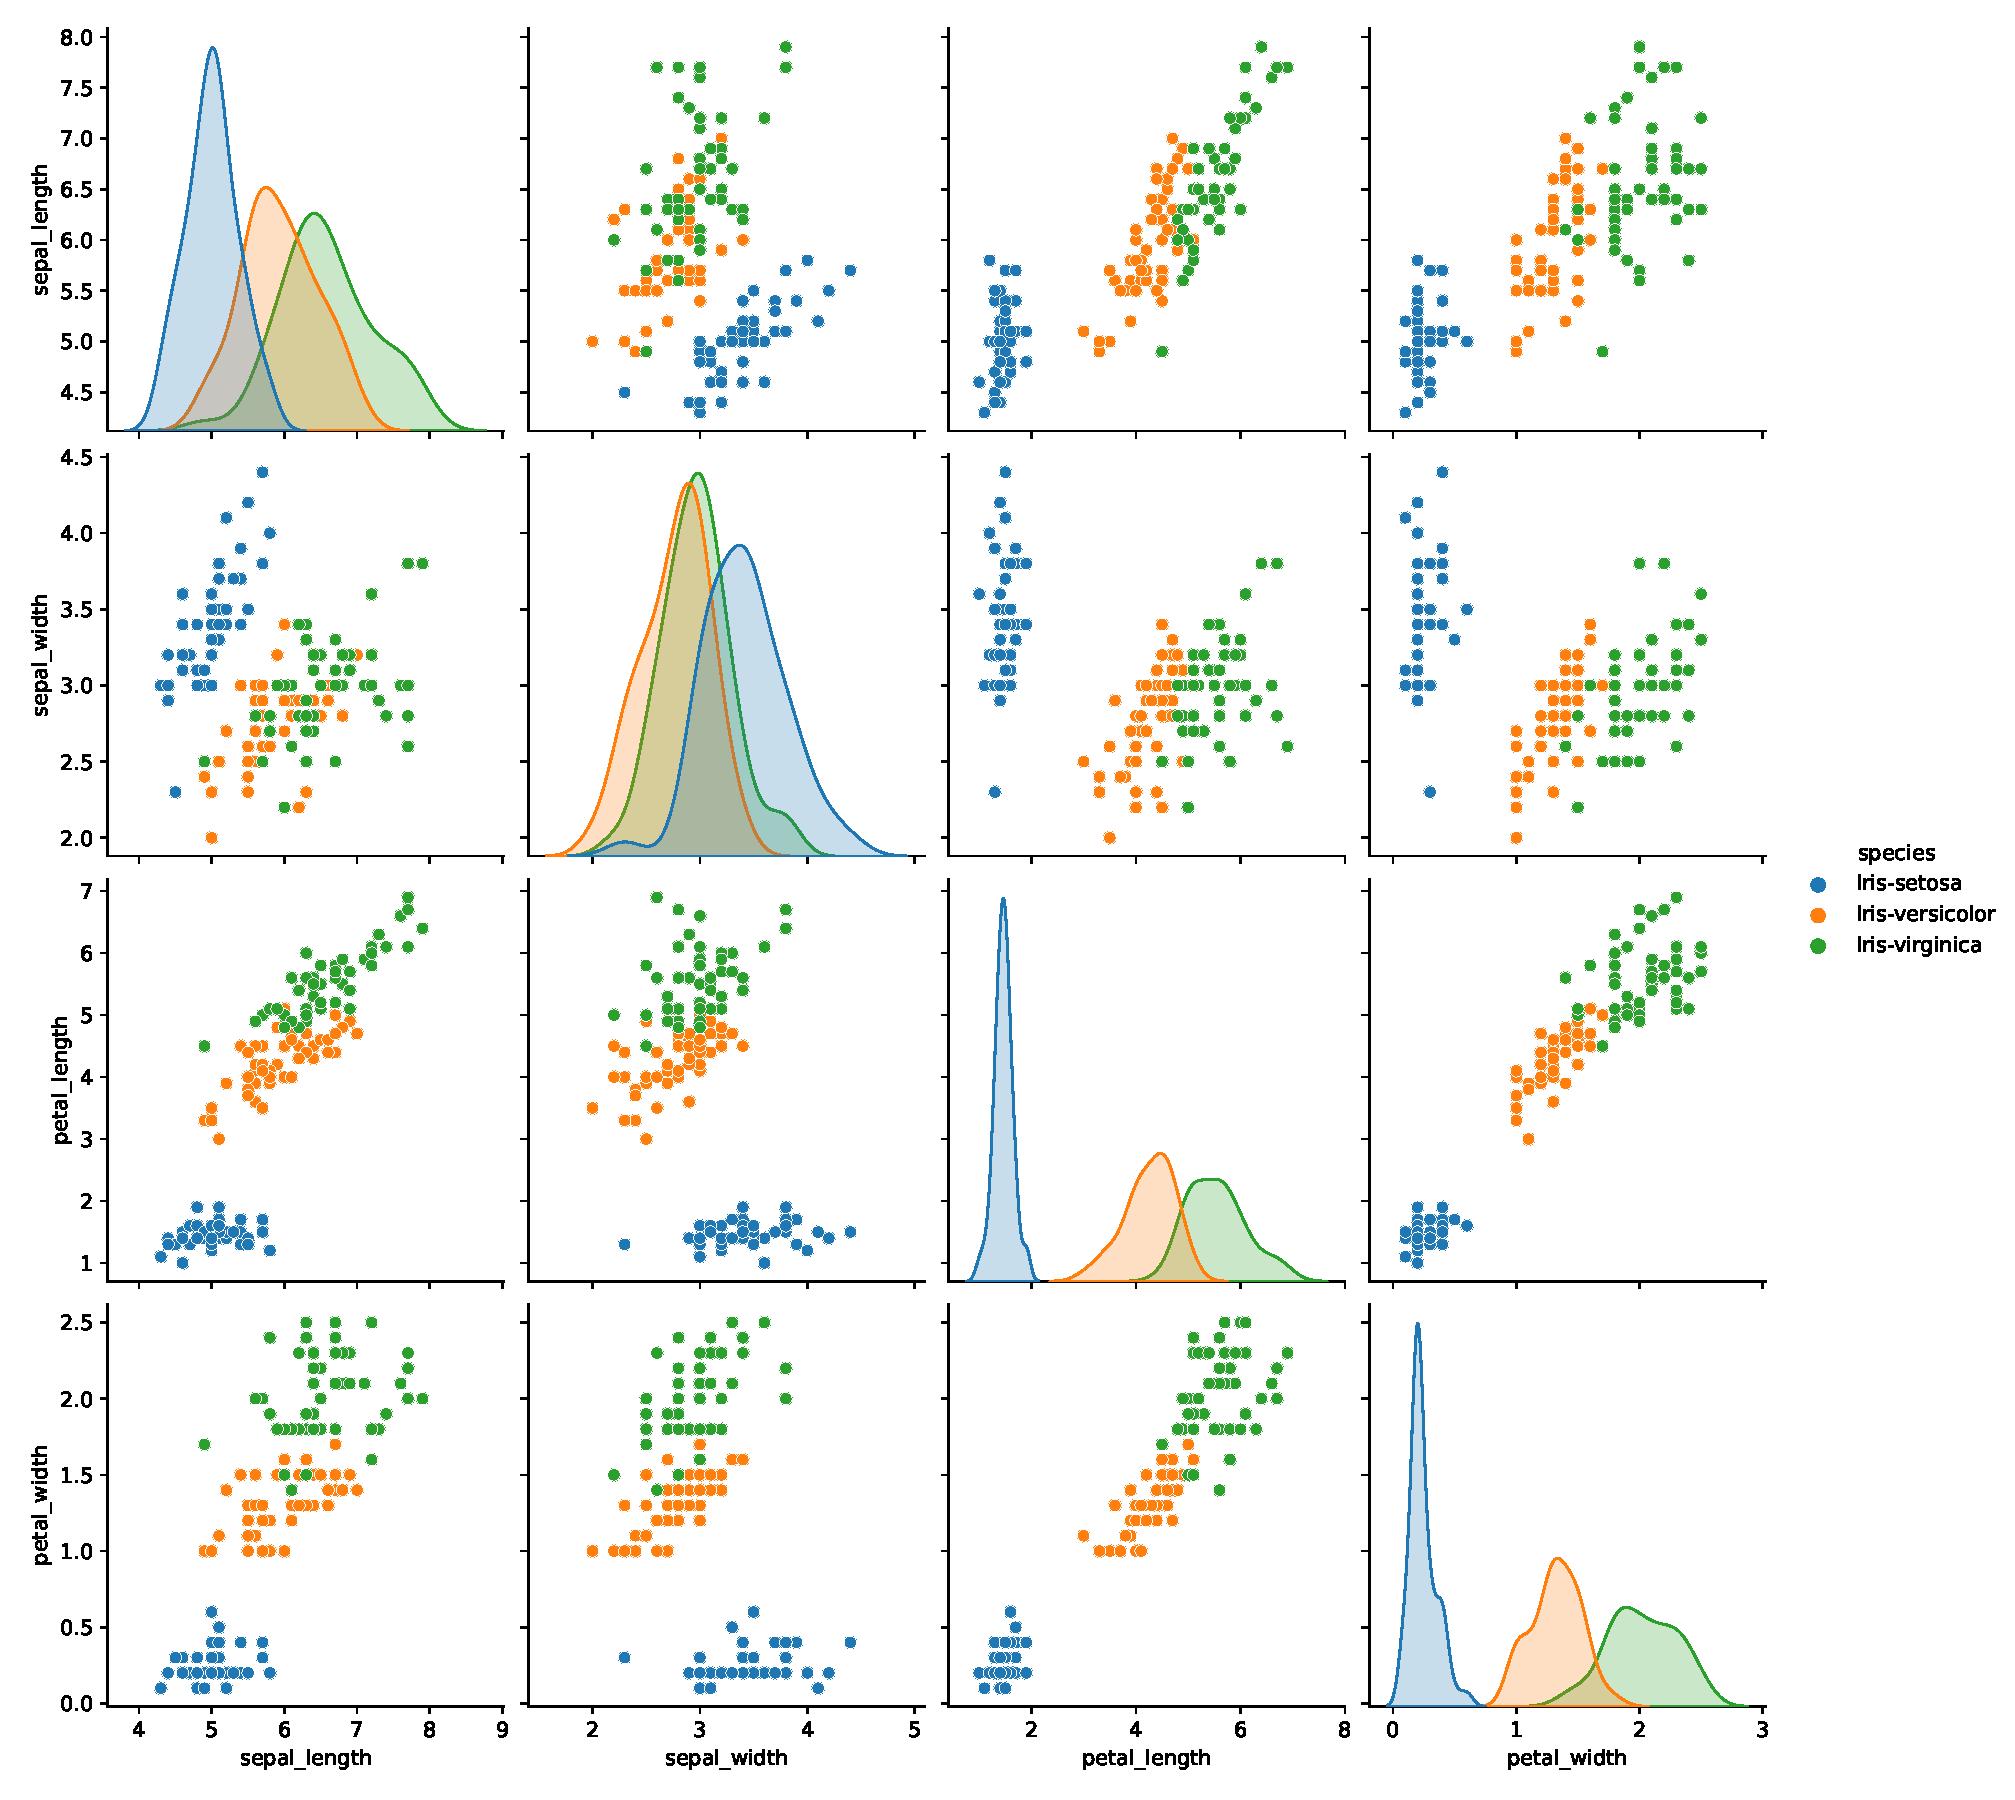
\includegraphics[width=0.7\linewidth]{../results/figures/figure.pdf}
    \legend{\footnotesize{\textbf{Notes:} XXX}}
    \end{figure}



\clearpage
\section{Appendix: Tables}

\begin{table}[htb]
    \vspace{0.5cm}
    \caption{Summary statistics}
    \label{tab:sumstat}
    \renewcommand{\arraystretch}{1.3}
    \small
    \begin{center}
    \input{../results/tables/my_table}
    \end{center}
    \end{table}


\end{appendix}
\end{document}



% Figure template

%\begin{figure}[htb]
%\centering
%\caption{Title of figure}\label{fig:figure_name}
%\vspace{2mm}
%\includegraphics[width=0.7\linewidth]{Name_of_file.pdf}
%\legend{\footnotesize{\textbf{Notes:} XXX}}
%\end{figure}


% Table template

%\begin{table}[htb]
%\vspace{0.5cm}
%\caption{Summary statistics}
%\label{tab:sumstat}
%\renewcommand{\arraystretch}{1.3}
%\small
%\begin{center}
%\input{tables/sumstat.tex}
%\end{center}
%\notes{XXX.}
%\end{table}
